\chapter{S4BXI class hierarchy}
\label{app:s4bxi_class_hierarchy}

\vspace{-10mm}

\begin{figure}[!ht]
    \centering
    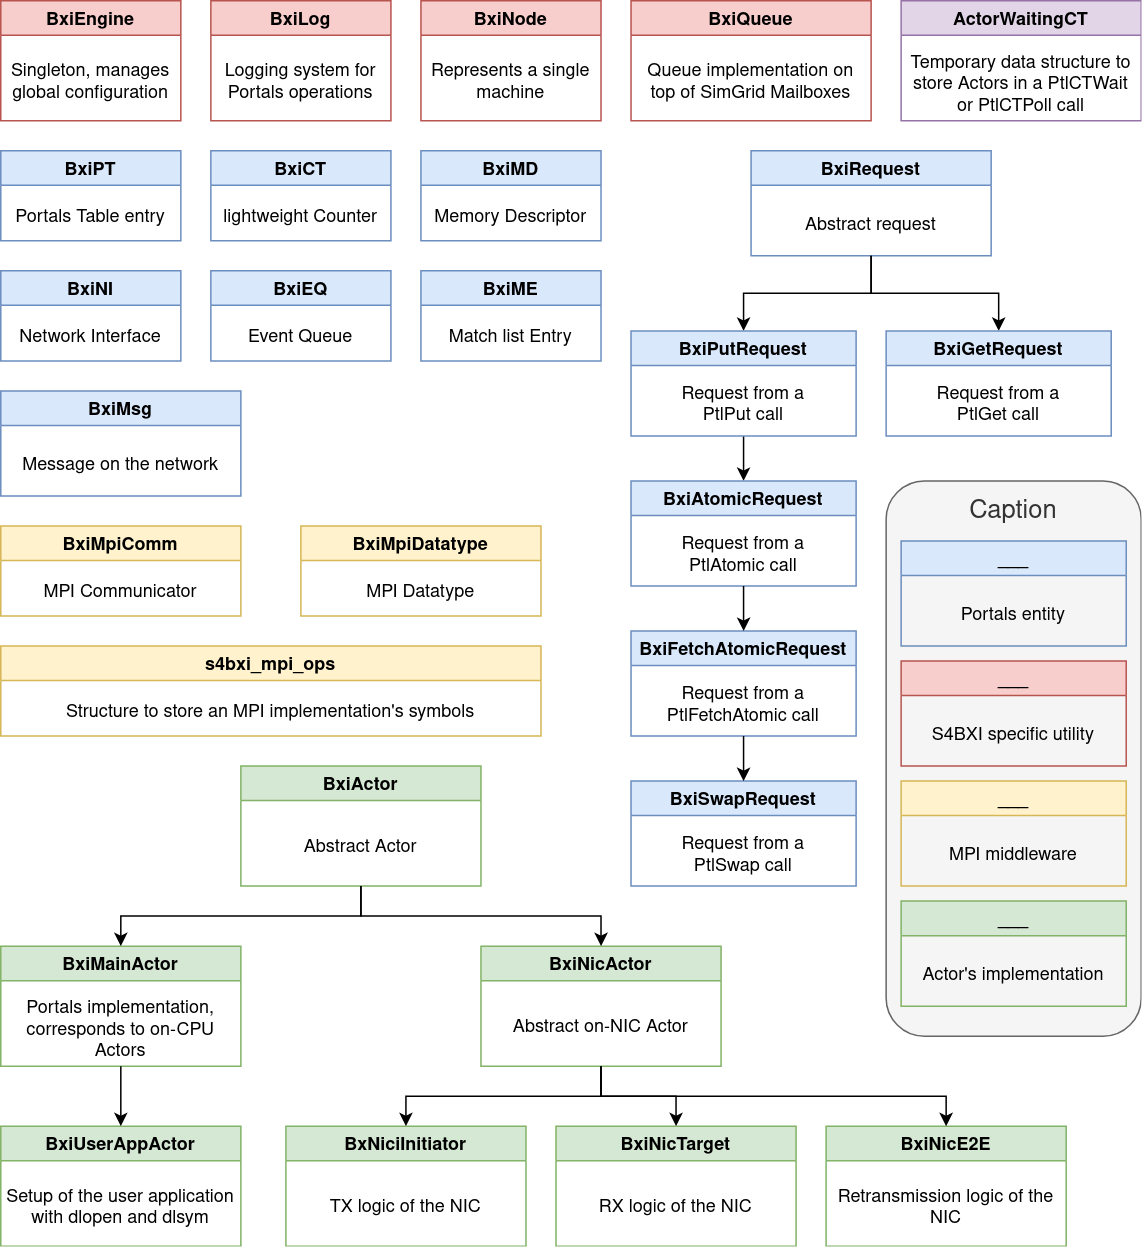
\includegraphics[width=\textwidth]{appendix/class_hierarchy.png}
    \caption{Full class hierarchy of our simulator}
    \label{fig:appendix:s4bxi_class_hierarchy}
\end{figure}

\makeatletter
\@openrightfalse
\makeatother

\chapter{OpenMPI patch}
\label{app:ompi_patch}

The following statistics where computed using cloc (\url{https://github.com/AlDanial/cloc}):

\begin{figure}[!ht]
    \lstinputlisting[basicstyle=\ttfamily\small,numbers=none]{appendix/cloc_diff_ompi.txt}
    \caption{Full statistics of our patch on OpenMPI to make it compatible with S4BXI (the Bourne Shell additions are simply small scripts we added to simplify the compilation, they are not meaningful modifications of the source code)}
    \label{fig:appendix:cloc_diff_ompi}
\end{figure}

\begin{figure}[!ht]
    \lstinputlisting[basicstyle=\ttfamily\small,numbers=none]{appendix/cloc_total_ompi.txt}
    \caption{Full statistics of OpenMPI after our patch}
    \label{fig:appendix:cloc_total_ompi}
\end{figure}

\chapter{OSU micro-benchmarks}
\label{app:osu_32}

Aggregated statistics of our OSU micro-benchmarks runs on 32 MPI ranks are shown
on Figure~\ref{fig:appendix:osu_32_time} for the accuracy of simulators, and
Figure~\ref{fig:appendix:osu_32_perf} for the slowdown compared to the
real-world run. The full data, for each MPI primitive, is available in the
following git repository:
\href{https://framagit.org/Webcretaire/phd-benchmark-data/-/tree/master/5_high_level/OSU}{https://framagit.org/Webcretaire/phd-benchmark-data}.

\begin{figure}[!ht]
    \centering
    \includegraphicsOverflow{appendix/OMPI_smpirun_8nodes4ppn_all.png}{1.15}
    \caption{Accuracy of SMPI and OpenMPI over S4BXI}
    \label{fig:appendix:osu_32_time}
\end{figure}

\begin{figure}[!ht]
    \centering
    \includegraphicsOverflow{appendix/OMPI_smpirun_8nodes4ppn_all_perf.png}{1.15}
    \caption{Slowdown of SMPI and OpenMPI over S4BXI}
    \label{fig:appendix:osu_32_perf}
\end{figure}

We can see that the IAllReduce benchmark is particularly pathologic for SMPI, as
it has a huge error and a very bad performance. The real-world experiment is
surprisingly quick for large message sizes (see
\url{https://framagit.org/Webcretaire/phd-benchmark-data/-/raw/master/5_high_level/OSU/32ranks/iallreduce_32.png}),
but our simulation method manages to model it accurately. These results seem to
indicate that the default algorithm used for this IAllReduce at this cluster
size is particularly bad for BXI in the community version of OpenMPI (which is
implemented in SMPI), and that it was optimized particularly well by Atos's
teams.

\chapter{S4BXI runtime for OpenSHMEM}
\label{app:oshmem_code}

\vspace{-1cm}
\lstinputlisting[multicols=2,xleftmargin=3mm,basicstyle=\ttfamily\scriptsize,language=C]{appendix/runtime-s4bxi.c}
